\documentclass{report}
\usepackage[a4paper]{geometry}
\usepackage{amsmath}
\usepackage{bm}
\usepackage{pgfplots}
\usepackage{ amssymb }
\usepackage{color, soul}
\usepackage[backend=biber]{biblatex}
\addbibresource{references.bib}
\graphicspath{{images/}}


%opening
\title{Directed Study Report\\CSE4DIR}
\author{Ash Hall\\17756156}

\newcommand{\TODO}[1]{\sethlcolor{pink}\hl{\\(#1)\\}}
\newcommand{\FEEDBACK}[1]{\sethlcolor{green}\hl{\\ Feedback: \\#1\\}}
\newcommand{\TOCITE}[2][citation needed]{\textsuperscript{\underline{#1}}}

\begin{document}

	\maketitle
	\thispagestyle{empty}
	\newpage
	\thispagestyle{empty}
	\tableofcontents
	\newpage
	\thispagestyle{empty}
	\newpage
	
	\setcounter{chapter}{1}	
	\chapter*{Directed Study Report}

	\section{Introduction}
	\TODO{This will be written properly once the rest is done}
	This report is about the effects of catastrophic interference in neural networks. \\
	We'll discuss some techniques for mitigating these effects, and will explore the severity of each.
	The benefit of exploring these things. \\
	
	
	\section{Transfer Learning}
	The training of a neural network occurs by presenting many examples, and iteratively optimising the weights. A dataset consisting of a small number of examples may be prohibitive to optimisation in this manner, as a model would likely over-fit to the training examples, and not be capable of generalising to novel examples. \emph{Transfer learning} minimising this problem, by allowing a pre-trained model to be re-purposed to a different dataset. \par
	The bulk of an image-classification neural network acts as a \emph{feature-extractor}, with studies\parencite{extractors} showing that a sufficiently-large image dataset leads to a highly-generalisable feature extractor. Transfer learning takes advantage of this property by taking the resultant feature extractor and amending the tail of a neural network to perform classification between different classes. Figure \ref{fig:transferlearning:1} shows a model pre-trained on a large image dataset being adapted to another. \par
	\begin{figure}[h]
		\centering
		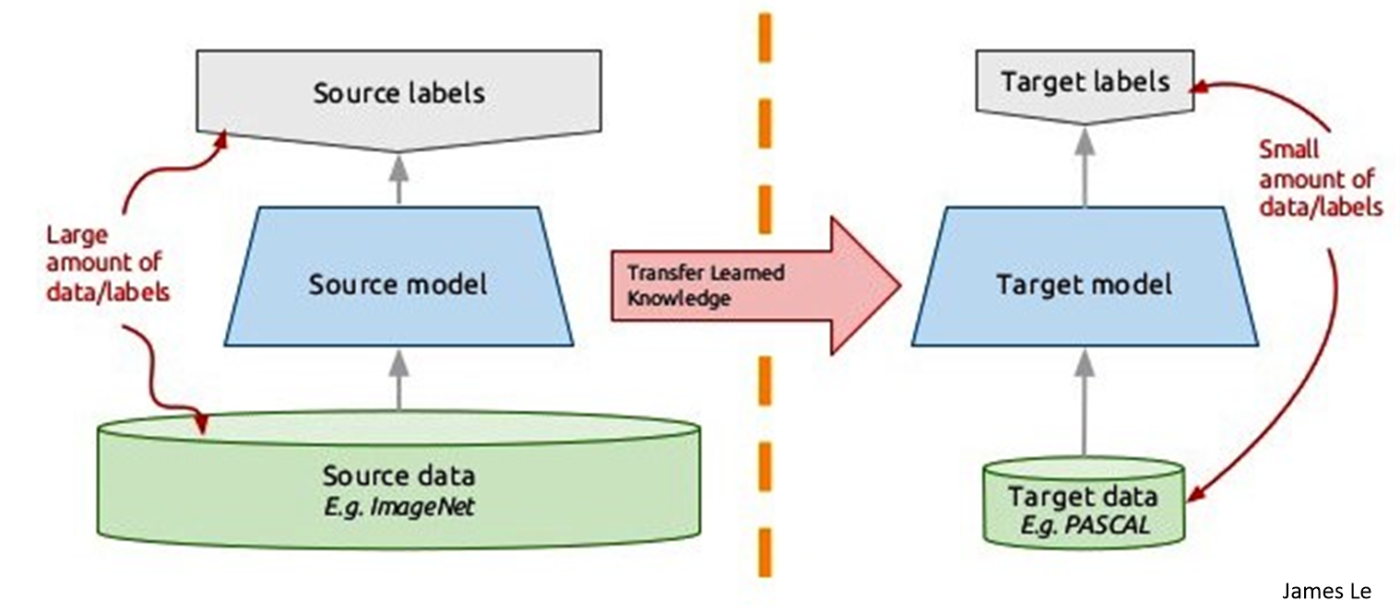
\includegraphics[width=11cm]{transferlearning}
		\caption{Transfer learning overview}
		\label{fig:transferlearning:1}
	\end{figure}
	There are two fundamental problems with this approach. The first is that although this lessens the effects of over-fitting, it doesn't entirely avoid them; training on a very small dataset is still prone to this problem. The other issue is that if you wished to not replace the old dataset classes, but add the new dataset classes to the model, you would need to store examples and repeatedly present them to the network during re-training. This introduces a whole suite of problems including training-example balancing, which we won't address here. \par
	Simply put, while providing strong results, transfer learning is limited in its usability, and is inherently inapplicable to the task of continuous learning -- which we'll address in the following section. \par
	
	\section{Continuous Learning}
	What continuous learning is. \\
	Why continuous learning is different to transfer learning (don't look at old examples) \\
	Briefly explain some techniques \\

	\subsection{Related Works}
	Intro to related works \\
	A few related works that address catastrophic interference	with continuous learning, why they're good and bad. \\
	Summary of related works \\

	\subsection{Environment}
	State the environment - (Ubuntu, docker, tensorflow etc.)
	
	\section{Framework}
	A description of the framework heirarchy. I'll give a simple diagram of the file-structure/python modules in the project, then explain roughly what everything is responsible for.
	
	\section{Training Procedure and Metrics}
	Here I'll explain how I trained each of the models (the stuff that's consistent between them), and give an introduction to some terms, and explain the metrics I used.
	
	\section{Benchmark Experiments and Results}
	I'll put a short introduction to the results here,
	
	\subsection{Experiment 1}
	(These will actually have names, not just experiment 1, 2, ...)
	\subsection{Experiment 2}
	\subsection{Experiment 3}
		
	\section{Summary}
	Summarise the experiment results and what impact they have on my project, summarise the work that I've done and where it leaves my with regards to the second semester and the "actual work". 
	
	
\end{document}
